\chapter{Technologies \& implémentations}
\label{Chapter3}

Ce chapitre reprend en détail chaque brique, en exposant pour chacune les recherches effectuées et des propositions de solutions pour leur implémentation ou mise en place.

\unsure{déplacer paragraphe ci-dessous ?}
Découvrant les domaines de l'urbanisme et de la modélisation du paysage avec la réalisation de ce projet, j'ai commencé par étudier les technologies et processus les plus répandus dans ces secteurs.

\section{Formats de fichiers 3D}

Dans le cadre de la mise en place d'une plateforme de partage de modèles 3D, l'étude des formats de fichiers existants (usages, tendances, compatibilité...) est un point de départ intéressant. Cela permet tout d'abord de découvrir comment sont représentées les données de modélisation, et comment elles se manipulent. On prend également connaissance des logiciels principaux du marché.

Au final, cela aidera à décider quel(s) format(s) seraient à considérer pour notre outil, celui-ci devant pouvoir \textbf{supporter les formats les plus courants} afin d'offrir une compatibilité maximale.

Il existe plus d'une centaine de formats permettant de stocker des données tridimensionnelles. De nombreuses listes de ces derniers sont disponibles sur internet, mais la plupart ne mentionnent que les principaux formats. La section consacrée à cette catégorie de fichiers sur \textit{Wikipédia}  \cite{wikipedia-3d-file-formats-list} s'avère être l'une des plus fournies. Un travail  de recherche sur ces formats et les logiciels associés offre également quelques indications utiles \cite{overview-of-3d-data-content}.

Cette abondance s'explique notamment par la variété des domaines concernés : de la représentation de structure moléculaires (format \textit{XYZ} \cite{xyz-format}), à la cryo-microscopie électronique (format \textit{MRC} \cite{mrc-format}), en passant par les formats de certains éditeurs de jeux ou consoles (\textit{MDX} chez \textit{Blizzard Entertainment}, \textit{BDL} et \textit{BMD3} chez Nintendo...), et bien entendu tous les logiciels de modélisation et d'animation (\textit{Blend} pour \textit{Blender}, \textit{FBX}, \textit{MAX}, \textit{MB} et bien d'autres pour les différentes suites proposées par \textit{Autodesk}, \ldots).

Dans le cadre de ce projet, les formats qui nous intéressent sont bien entendu ceux qui concernent l'urbanisme, au travers des logiciels de CAO/DAO correspondants.

Enfin, il est important de savoir qu'un fichier 3D n'est pas qu'une simple liste de coordonnées 3-axes, mais contient généralement de nombreuses autres informations telles que : 
\begin{itemize}
    \item Caméras : types de caméra, angle, position...
    \item Lumières : types, emplacements, effets...
    \item Maillages (\textit{meshes}),
    \item Textures,
    \item Animations, sons...
\end{itemize}

Le contenu exact varie beaucoup d'un format à l'autre. Aussi, là où un certain format permettra de stocker l'ensemble des informations d'un modèle, un autre nécessitera de séparer les données (par exemple, un fichier pour la structure générale du modèle, et un autre pour les textures et le matériel). Des exemples de cela seront donnés au fur et à mesure des descriptions qui suivent.

Avant de débuter un tour d'horizon des principaux formats, nous commençons par un petit aparté sur un consortium qui sera mentionné régulièrement.

\subsection{Khronos Group}
\label{sec:khronos-group}
Le \textit{Khronos Group} est un consortium industriel à but non lucratif, dont le but est de définir des standards ouverts et libres de droits dans les domaines des graphiques 3D, de la réalité virtuelle et augmentée, et du traitement d'images notamment. Il maintient de nombreuses technologies, comme \textit{OpenGL}, \textit{WebGL} ainsi que des formats de fichiers 3D dont cetains seront présentés en \ref{sec:main-3d-file-formats}.

La figure \ref{fig:khronos-visual-computing-ecosystem} présente l'écosystème des standards proposé par le groupe.

\begin{figure}[h]
    \centering
    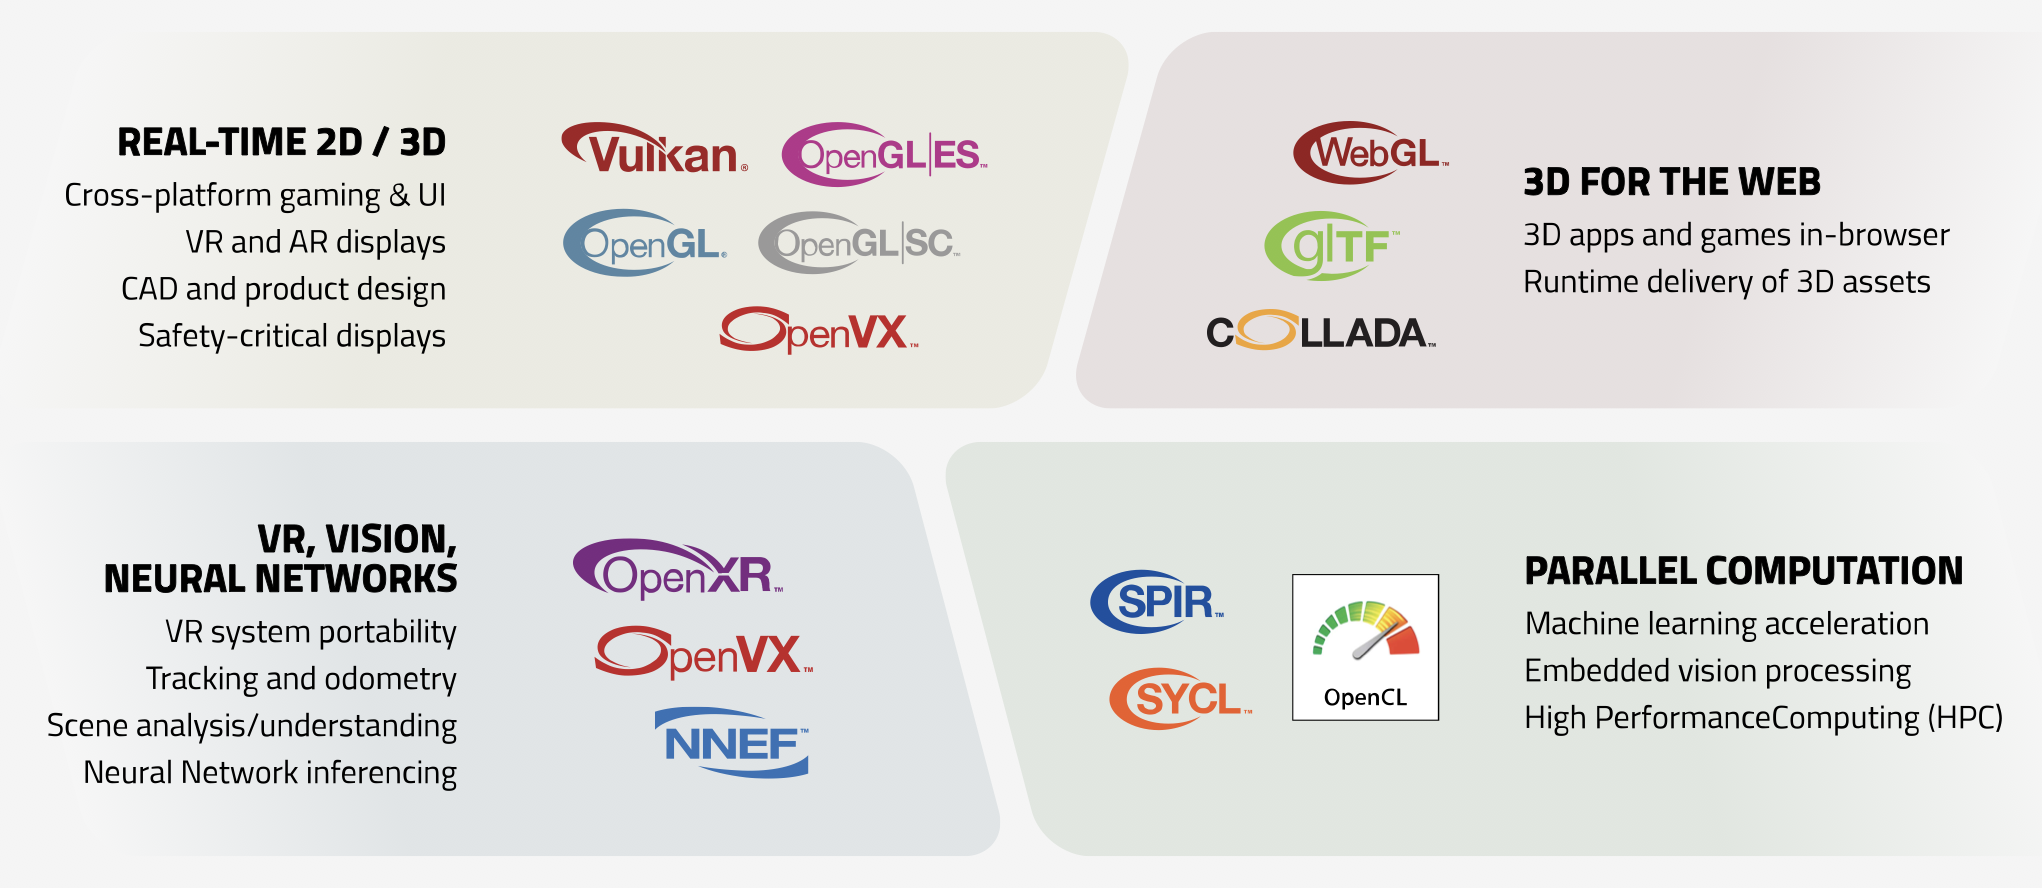
\includegraphics[width=0.8\linewidth]{Figures/khronos-visual-computing-ecosystem.png}
    \captionsource{Ecosystème des standards proposés par \textit{Khronos}.}{khronos-ecosystem}
    \label{fig:khronos-visual-computing-ecosystem}
\end{figure}

\subsection{Formats de fichiers de DAO/CAO courants}
\label{sec:main-3d-file-formats}

Cette section présente les formats de données 3D les plus représentés sur le marché actuellement.

\subsubsection{FBX}
\textit{FBX} (\textit{\textbf{F}ilm\textbf{b}o\textbf{x}}) est un format appartenant à \textit{Autodesk}.

Bien que propriétaire, une \textit{API} fournit le nécessaire pour lire et écrire ces fichiers \cite{fbx-api}.

Il a été créé pour pallier les variétés de formats rencontrés dans le flux de travail, et ainsi assurer l'interopérabilité entre les produits d'\textit{Autodesk}, tels que \textit{3ds Max}, \textit{Maya} ou \textit{Motion Builder}, ainsi que de nombreux autres logiciels comme \textit{Cinema4D}, \textit{Rhino} ou \textit{Unity3D}.

De fait, cela en fait un format populaire, très répandu.
Une rapide recherche sur \textit{GitHub}\footnote{\url{https://github.com/search?q=fbx+viewer}} nous renvoie de nombreux projets de visionneuses \textit{FBX}.

\subsubsection{OBJ}
\textit{OBJ} est un format libre très utilisé pour transférer des informations d'une application à l'autre. Il s'agit d'un format de données simple, en \textit{ASCII}, qui sert uniquement à représenter la géométrie 3D (\textit{mesh}).

Comme ce format n'inclut pas les informations de couleurs, matériel, transformation et consort, un fichier \textit{MTL} (\textit{\textbf{M}aterial \textbf{T}emplate \textbf{L}ibrary}) lui est généralement associé. Ce dernier définit les matériaux d'un objet 3D (coloration, texture, paramètres de réflexions optique...). Malheureusement \textit{MTL} est un format dépassé au vue des technologies actuelles, dont il ne supporte pas les plus récentes.

\subsubsection{3ds}
\textit{3ds} est l'un des formats utilisé par \textit{Autodesk 3ds Max}. Format natif du logiciel depuis son origine dans les années 90, cela en fait également un format très utilisé pour partager des modèles. Comme son concurrent \textit{OBJ}, il nécessite des fichiers complémentaires (\textit{MAX} pour stocker toutes les informations de la scène.

\subsubsection{COLLADA}
\textit{COLLADA} (\textit{\textbf{COLLA}borative \textbf{D}esign \textbf{A}ctivity})\footnote{\url{https://www.khronos.org/collada}} a intialement été développé par \textit{Sony Computer Entertainment}, et appartient actuellement au \textit{Khronos Group} \cite{collada-format}.
C'est un format libre, dont la spécification est décrite par une norme ISO \cite{collada-iso}.

Il a été conçu pour faciliter les échanges entre les différents logiciels. Les documents \textit{COLLADA} décrivent les éléments selon un schéma \textit{XML}, et portent généralement l'extension \textit{DAE} (\textit{\textbf{D}igital \textbf{A}sset \textbf{E}xchange}.

Ce format est listé comme inactif dans la liste des standards du \textit{Khronos Group}. 
Bien que cela ne soit pas encore déclaré de façon officielle, il semble que le format \textit{glTF}, présenté en \ref{sec:glTF}, lui succède.

\subsubsection{glTF}
\label{sec:glTF}

\textit{glTF} (\textit{\textbf{GL} \textbf{T}ransmission \textbf{F}ormat}) est autre un standard ouvert défini par le \textit{Khronos Group} \cite{gltf-format}. Visant le même objectif que son prédécesseur \textit{COLLADA}, ce format a été optimisé au mieux pour réduire l'espace de stockage nécessaire pour les scènes ou modèles 3D représentés, tout en accélérant le chargement et traitement de ceux-ci. 
\textit{Khronos} le décrit comme le "JPEG de la 3D".
Ce format utilise \textit{JSON} pour décrire les données.

Bien que relativement récent (fin 2015), il a rapidement été adopté par les principaux acteurs du marché, et son acceptation continue de s'étendre. À titre d'exemple, \textit{Sketchfab} propose déjà plus de 100'000 modèles dans ce format \cite{sketchfab-largest-gltf-repository} et a défini \textit{glTF} comme format d'exportation par défaut. Tous les modèles, quelque soit leur format d'origine, peuvent être convertis automatiquement dans ce format lors de leur téléchargement. 

\begin{figure}
    \centering
    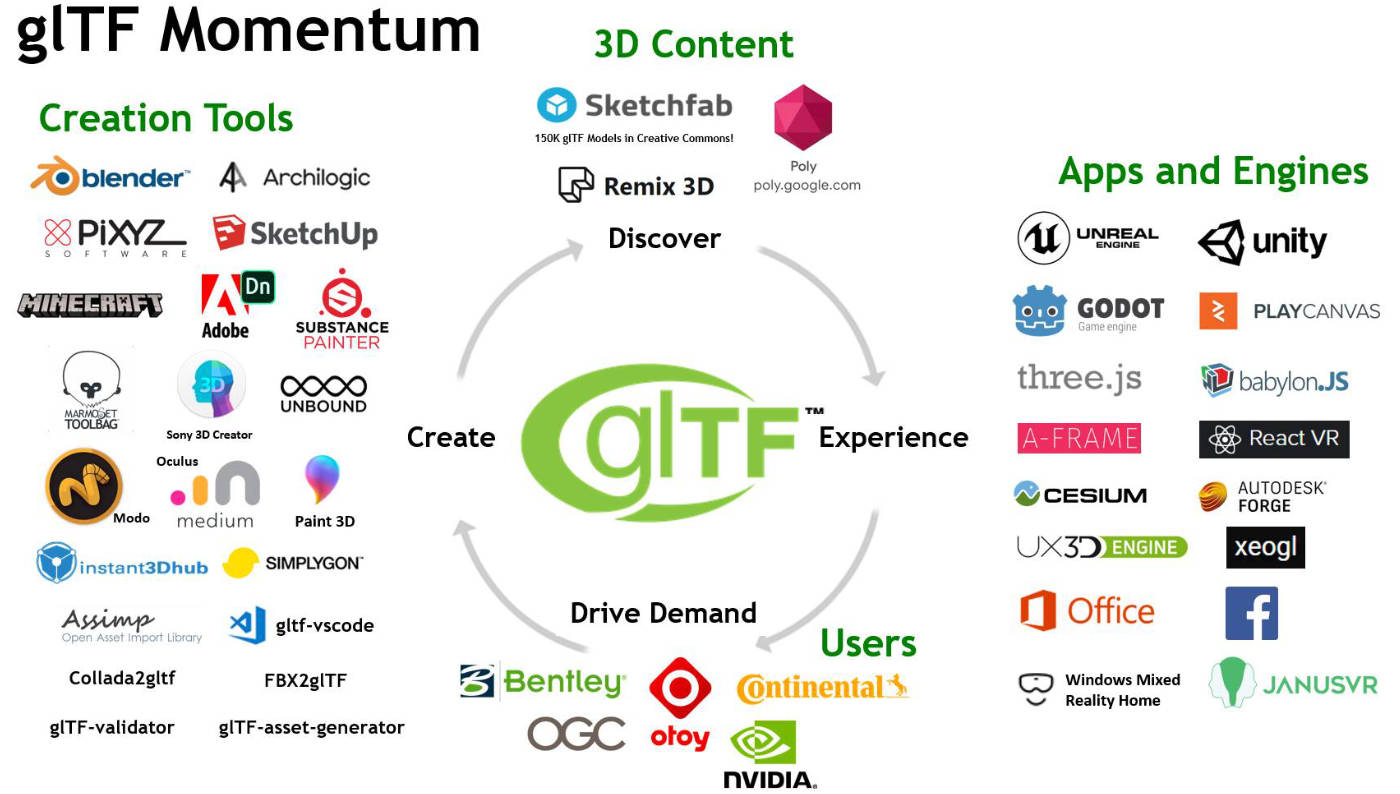
\includegraphics[width=0.8\linewidth]{Figures/gltf-momentum.jpg}
    \captionsource{Outils, applications, plateformes et sociétés employant \textit{glTF}}{gltf-momentum}
    \label{fig:gltf-momentum}
\end{figure}

\subsection{Supports des formats dans le cadre du projet}

Une première possibilité, illustrée par la figure \ref{fig:file-importation-process-native}, est de faire en sorte que l'outil sache lire les fichiers "tels quels", sans effectuer de réelles transformations.
L'avantage est que, pour autant que l'on ait implémenté le support du format de fichier fournit en entrée, celui-ci sera rendu correctement. C'est le principe employé par la plupart des visionneuses d'images. Elles intègrent les spécifications de chaque format supporté, et affichent correctement chaque pixel à l'écran.
Le problème de cette solution est qu'elle nécessite un travail conséquent, proportionnel au nombre de formats que l'on souhaite implémenter, de mise en place des spécifications de ceux-ci et de vérification que le rendu est effectué correctement pour chacun.

\begin{figure}[ht]
    \centering
    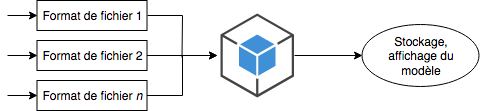
\includegraphics[width=0.7\linewidth]{Figures/file-importation-process-native.png}
    \caption{Cas 1 : support natif des principaux formats}
    \label{fig:file-importation-process-native}
\end{figure}

Une seconde option, représentée par la figure \ref{fig:file-importation-process-manual-conversion}, consiste à ne définir que quelques (voire un seul) formats principaux, qui seront supportés par le logiciel. Si l'utilisateur souhaite importer un modèle réalisé dans un format non pris en charge, il devra le convertir manuellement, par exemple à l'aide des fonctions d'exportation du logiciel utilisé pour sa conception. Cela nécessite un temps de développement réduit par rapport à la première solution. Il convient cependant de bien sélectionner les formats retenus, afin de limiter les cas où l'utilisateur doit effectivement procéder à une conversion préalable.

\begin{figure}[ht]
    \centering
    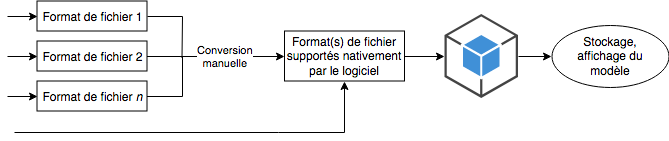
\includegraphics[width=0.9\linewidth]{Figures/file-importation-process-manual-conversion.png}
    \caption{Cas 2 : conversion manuelle vers le(s) format(s) supportés}
    \label{fig:file-importation-process-manual-conversion}
\end{figure}

Enfin, la troisième possibilité, qu'illustre la figure \ref{fig:file-importation-process-auto-conversion}, est une variante de la seconde. Cette fois, si le format de fichiers en entrée n'est pas de ceux que le logiciel sait manipuler directement, une conversion automatique est réalisée. Évidemment, cela suppose que la fonction de conversion nécessaire du format \textit{X} vers un format supporté ait été implémentée. Cela reste néanmoins assez aisé, car les principaux standards proposent des \textit{API} de conversion, facilitant ce travail. Cette option reste plus simple à mettre en place que la première, tout en étant plus agréable pour l'utilisateur que la seconde, car il n'a plus à se préoccuper de convertir à chaque fois son modèle lui-même s'il utilise un logiciel employant un autre format.

\begin{figure}[ht]
    \centering
    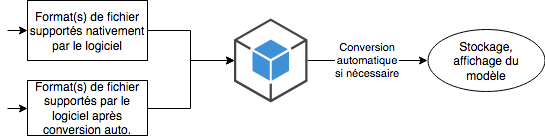
\includegraphics[width=0.8\linewidth]{Figures/file-importation-process-auto-conversion.png}
    \caption{Cas 3 : conversion effectuée par le logiciel, si nécessaire}
    \label{fig:file-importation-process-auto-conversion}
\end{figure}

Le troisième cas de figure est l'option privilégiée dans les logiciels de CAO. La plupart intègrent en effet des modules d'importation, et également d'exportation, de et vers de multiples formats.
La conversion n'est généralement pas implicite, et nécessite que l'utilisateur active l'outil correspondant. Mais c'est bien le logiciel lui-même qui effectue l'opération.

Pour notre plateforme, il paraît évident que cette option serait à privilégier. Cependant, le prototype est basé sur le cas 2 (conversion manuelle préalable), pour les raisons présentées dans la section \ref{sec:3d-model-viewers}.

\section{Visionneuses de modèles 3D}
\label{sec:3d-model-viewers}

L'affichage et la manipulation de modèles 3D constitue la première brique de notre outil, la fondation sur laquelle viendront s'ajouter les modules complémentaires souhaités, tels que la gestion d'annotations, le stockage des modèles et des notes associées, etc.

Il existe de multiples visionneuses, qu'elles soient hébergée en ligne ou à installer.
Les critères suivants ont été définis pour affiner la sélection :

\begin{itemize}
    \item \textbf{\textit{Open-source}} : condition nécessaire dans le cadre d'un projet comme celui-ci où l'on cherche à partir de bases existantes que l'on assemble, et visant un but collaboratif.
    \item Formats : la visionneuse doit supporter un ou plusieurs formats de fichiers 3D parmi les plus répandus actuellement.
    \item Actuel : le projet doit être récent, et si possible toujours actif, afin de garantir qu'il utilise des technologies récentes et augmenter les chances qui continue d'être développé.
\end{itemize}

Voici les projets qui présélectionnés :

\begin{itemize}
    \item \textbf{bwasty/gltf-viewer}\footnote{\url{https://github.com/bwasty/gltf-viewer}}: développée en \textit{Rust}, cette visionneuse est fonctionnelle, mais n'a pas été retenue, d'une part car elle ne propose pas de version web, et d'autre part car c'est un langage dans lequel nous n'avons pas d'expérience.
    
    \item \textbf{pissang/clay-viewer}\footnote{\url{https://github.com/pissang/clay-viewer}} : cette visionneuse permet de lire les fichiers \textit{FBX}, \textit{DAE} et \textit{OBJ}, et il est ensuite possible de les exporter au format \textit{glTF}. Les versions clients Windows et MacOS sont proposées. Très prometteur, ce projet n'a pas été retenu comme base pour deux raisons. La première, c'est qu'il n'est pas fait mention de version web - bien qu'en théorie, au vu des technologies utilisées (\textit{Javascript}, principalement), il serait possible de l'adapter. La seconde, c'est que le rendu est effectué à l'aide de ClayGL\footnote{\url{https://github.com/pissang/claygl}}, une librairie créée par le même développeur. Celle-ci est très prometteuse, maintenue activement à jour et commence à être utilisée dans quelques projets, mais n'est pas encore suffisamment répandue pour assurer que l'on trouvera suffisamment de documentation, exemples et aide en cas de besoin.
    À noter que ce projet propose un outil de conversion vers glTF, fait en python, dont on pourrait se servir.
    
    \item \textbf{three-gltf-viewer}\footnote{\url{https://github.com/donmccurdy/three-gltf-viewer}}: il s'agit d'une visionneuse de fichiers \textit{glTF} uniquement. Ce qui peut apparaître comme un inconvénient est compensé par le fait que le projet est web, utilise des technologies répandues, et est simple à utiliser. De plus, comparé à ses concurrents, le rendu des modèles est plus précis. C'est ce projet qui a été retenu. Il est décrit en \ref{sec:three-gltf-viewer}.
\end{itemize}

\subsection{Three-gltf-viewer}
\label{sec:three-gltf-viewer}

\textit{Three-gltf-viewer} est une visionneuse de fichiers \textit{gltf}, activement développée par un passionné de chez \textit{Google} travaillant dans la visualisation.

Il s'agit d'un projet multiplateformes, pouvant fonctionner dans un navigateur, mais dont on peut également générer une version cliente pour \textit{Windows}, \textit{MacOS} et \textit{Linux}.

Son principe est simple : une fois chargée, l'application demande à l'utilisateur de fournir son modèle \textit{glTF}, simplement par glisser-déposer. Celui-ci est alors affiché à l'écran et navigable (zoom, rotation...).

Le rendu est bien réalisé, contrairement à celui effectué par \textit{clay-viewer} par exemple, comme le montre la figure \ref{fig:clay-viewer-vs-three-gltf-viewer}. 

\begin{figure}[h]
    \centering
    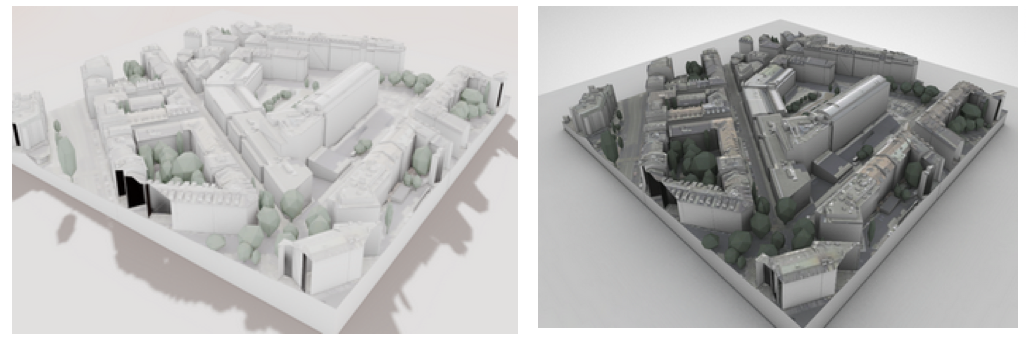
\includegraphics[width=\linewidth]{Figures/clay-viewer-vs-three-gltf-viewer.png}
    \caption{Comparaison de rendu entre \textit{clay-viewer} (gauche) et \textit{three-gltf-viewer} (droite)}
    \label{fig:clay-viewer-vs-three-gltf-viewer}
\end{figure}

L'une des contraintes lorsque l'on se base sur un projet existant, est qu'il va falloir s'adapter aux technologies que celui-ci emploie.

Un rapide tour d'horizon sur la page \textit{GitHub} du projet, en affichant la proportion d'utilisation des langages comme illustré par la figure \ref{fig:three-gltf-viewer-github-preview}, nous apprend que le code est essentiellement écrit en \textit{JavaScript}. S'agissant d'une application web, cela n'est guère suprenant.

\begin{figure}[h]
    \centering
    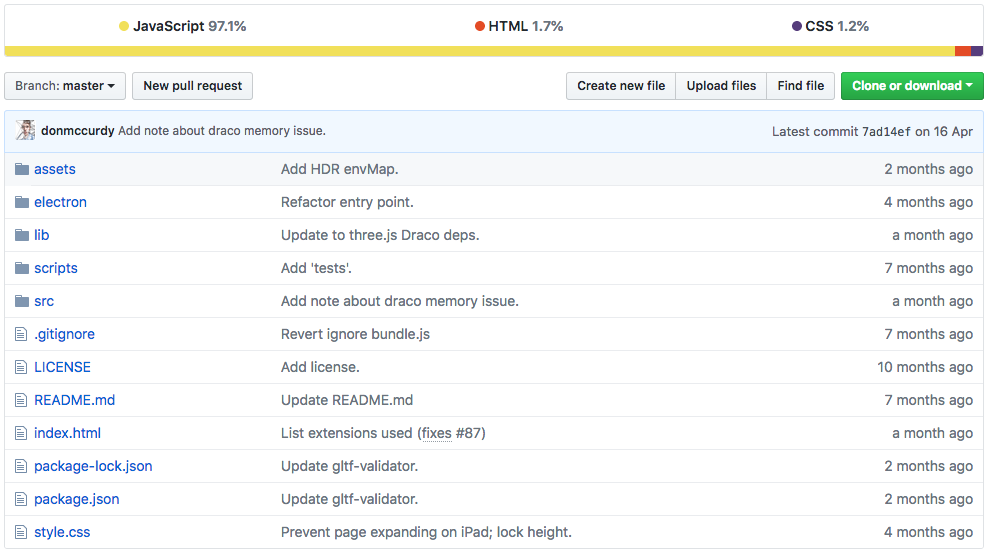
\includegraphics[width=\linewidth]{Figures/three-gltf-viewer-github-preview.png}
    \caption{Statistiques du projet three-gltf-viewer}
    \label{fig:three-gltf-viewer-github-preview}
\end{figure}

Le projet utilise également plusieurs librairies décrites ci-après.

\subsubsection{WebGL}

\begin{wrapfigure}{r}{0.3\textwidth}
  \begin{center}
    
\includegraphics[width=0.28\textwidth]{Figures/webgl-logo.png}
  \end{center}
\end{wrapfigure}
\textit{WebGL} est une API, basée sur \textit{OpenGL}, servant à afficher des graphiques 2D et 3D dans tout navigateur web compatible\cite{webgl-compatibility}, à travers le \textit{canvas} d'\textit{HTML5}. 
Le rendu, au travers du langage \textit{GLSL}, est réalisé par le \textit{GPU}, fournissant ainsi d'excellentes performances. Ces dernières peuvent toutefois être limitées, par exemple sur des ordinateurs équipées d'anciennes cartes graphiques ainsi que les smartphones à la configuration plus modeste.

\textit{WebGL} est développé par le groupe \textit{Khronos}, le même à l'origine du format \textit{glTF} présenté en \ref{sec:glTF}.

\subsubsection{Three.js}

\begin{wrapfigure}{r}{0.25\textwidth}
  \begin{center}
    
\includegraphics[width=0.23\textwidth]{Figures/threejs-logo.png}
  \end{center}
\end{wrapfigure}

\textit{Three.js} est une librairie \textit{JavaScript} libre, permettant de créer et afficher des éléments 3D dans un navigateur. Très répandue, elle s'utilise facilement dans un document \textit{HTML5}, typiquement à l'aide de la balise \texttt{canvas}.

La librairie fonctionne dans tout navigateur compatible \text{WebGL} et propose de nombreuses fonctionnalits pour la gestion des scènes, de l'éclairage, du matériel, des animations, etc.

La documentation en ligne comprend de nombreux exemples permettant de démarrer rapidement.

\textit{Three-gltf-viewer} fait usage de \textit{Three.js} pour afficher et manipuler les modèles 3D.

\subsubsection{Node.js}

\begin{wrapfigure}{r}{0.25\textwidth}
  \begin{center}
    
\includegraphics[width=0.23\textwidth]{Figures/nodejs-logo.png}
  \end{center}
\end{wrapfigure}

\textit{Node.js} est un environnement d'exécution \textit{Javascript} multiplateformes \textit{open-source} très largement répandu, qui exécute le code \textit{JavaScript} côté serveur.

Dans le cadre de \textit{three-gltf-viewer}, il sert à déployer la version web de l'application.

\subsubsection{Electron}

\begin{wrapfigure}{r}{0.23\textwidth}
  \begin{center}
    
\includegraphics[width=0.21\textwidth]{Figures/electron-logo.png}
  \end{center}
\end{wrapfigure}

\textit{Electron} est une librairie \textit{open-source} développée par \textit{GitHub} permettant de développer des applications clientes multi-plateformes (\textit{Windows}, \textit{Linux} et \textit{macOS}) avec \textit{JavaScript}, \textit{HTML} et \textit{CSS}. De nombreux logiciels l'utilisent, parmi lesquels \textit{Slack}, \textit{Skype}, \textit{Atom}, \textit{Microsoft Visual Studio Code} ou encore la version bureau de \textit{Whatsapp}. 

Dans le cas de \textit{three-gltf-viewer}, les binaires pour toutes les plateformes peuvent être générés en appelant simplement la commande \texttt{npm run package} (\texttt{package} étant un script défini par l'auteur du projet, qui va appeler les instructions correspondantes).

\section{Annotations}

Lors de l'analyse préliminaire, il a notamment été mis en évidence l'importance d'une fonctionnalité d'annotation. Dans le cadre de ce projet, ces annotations ont la particularité d'être \textbf{associées à des coordonnées spécifiques du modèle 3D}. Ce ne sont donc pas de simples commentaires ajoutés par exemple en regard du modèle ou en dessous de celui-ci, comme cela est généralement fait lorsque l'on commente des photos ou une publications d'un réseau social, par exemple.

\subsection{Attributs d'une annotation}

Une annotation se définit principalement par son \textbf{contenu} ainsi que sa \textbf{localisation dans le modèle}.

Par contenu, on pense généralement à du texte mais, comme cela a été présenté dans la section \ref{sec:global-architecture} ainsi qu'illustré avec la figure \ref{fig:various-media-for-annotation}, cela peut tout aussi bien être des images, des liens web, une vue 360° prise à l'emplacement concerné, une vidéo, une vue en coupe, voire un autre modèle 3D (par exemple, l'intérieur d'un bâtiment)...!

Dans \textit{Sketchfab}, les annotations ont un titre et une description. Cette dernière peut être rédigée en \textit{Markdown}; c'est de cette manière que l'on peut également y adjoindre des liens et des images, ces dernières devant alors être stockées sur un autre service.
Pour l'instant, la plateforme ne supporte pas les autres types de médias.

\begin{figure}
    \centering
    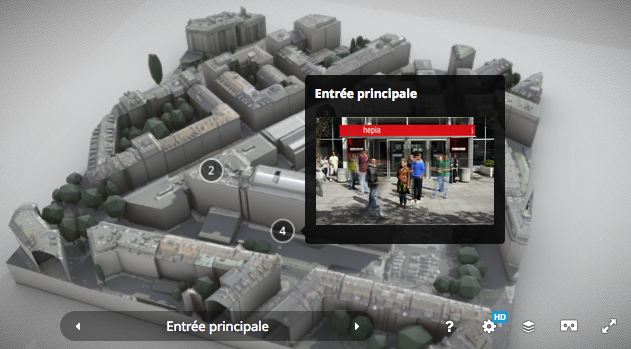
\includegraphics[width=0.9\linewidth]{Figures/sketchfab-annotation-with-picture.png}
    \caption{Exemple d'annotation avec une image dans~\textit{Sketchfab}}
    \label{fig:sketchfab-annotation-with-picture}
\end{figure}

\subsection{Utilisation}

L'ajout d'une annotation dans \textit{Sketchfab} se déroule ainsi : 
\begin{itemize}
    \item Ouvrir le modèle en mode édition et activer l'outil d'annotation.
    \item Effectuer un double-clic sur le modèle à l'emplacement désiré : une fenêtre de saisie s'affiche.
    \item Une fois l'annotation validée, celle-ci est représentée par un cercle numéroté, qui reste à l'emplacement choisi, même lorsque l'on manipule le modèle (rotation, déplacement...).
\end{itemize}

\begin{figure}[h]
    \centering
    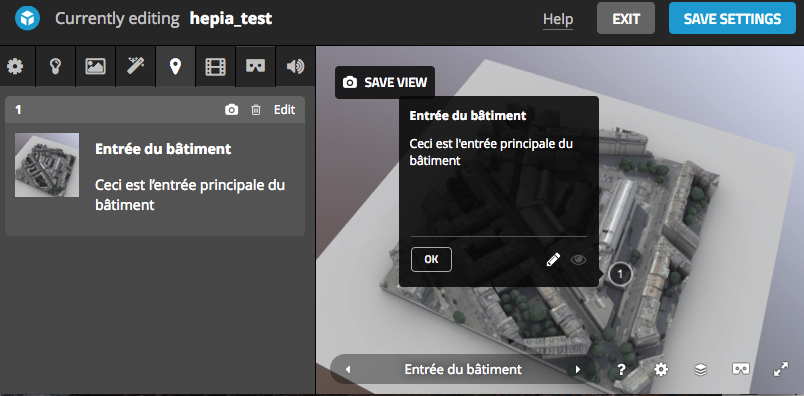
\includegraphics[width=0.9\linewidth]{Figures/sketchfab-adding-annotation.png}
    \caption{Exemple d'ajout d'une annotation en mode édition}
    \label{fig:sketchfab-adding-annotation}
\end{figure}

Pour afficher une annotation, il suffit de cliquer sur son marqueur dans le modèle.

C'est une façon de faire simple et facilement compréhensible par l'utilisateur.

\subsection{Implémentation}

Le cercle ou point indiquant l'existence et l'emplacement d'une annotation sur le modèle est généralement un objet 3D ajoutés à la scène rendue en \textit{WebGL}. De cette manière, les opérations effectuées par l'utilisateur, telle une rotation, sont répercutées à la fois sur le modèle et les marqueurs d'annotations, permettant à ces dernières de conserver leur position relativement au modèle.

Le dialogue permettant de créer, modifier ou afficher l'annotation est, lui, généré à l'aide d'\textit{HTML/CSS}, bien mieux adaptés pour tout ce qui a trait à la mise en page et aux typographies. Ses coordonnées, 2D, sont calculées par rapport à la fenêtre du navigateur. Afin de pouvoir l'afficher en regard du marqueur de l'annotation et pouvoir suivre celui-ci en cas de manipulation du modèle, il est nécessaire de mettre à jour les coordonnées du dialogue en effectuant une conversion du monde 3D de la scène, vers la 2D du navigateur. Cette opération s'appelle une \textbf{projection}. \textit{Three.js} fournit une fonction \texttt{project} à cet effet.

À l'inverse, lorsque l'on clique sur la scène pour ajouter une annotation, il faut convertir les coordonnées 2D de l'emplacement du curseur dans le navigateur, vers les coordonnées 3D correspondantes dans la scène afin de déterminer où, et sur quel élément l'action a été réalisée.
La figure \ref{fig:mip-viewer-raycasting-code} illustre le code correspondant. Lorsque l'on clique sur le modèle, un \textit{raycasting} est réalisé : un trait imaginaire est "tiré" dans le monde 3D depuis l'emplacement cliqué, et si une collision avec un objet de la scène se produit, celui-ci est retourné. C'est ainsi que l'on reconnaît un clic sur un marqueur d'annotation, d'un clic sur le modèle lui-même, par exemple.

\begin{figure}
    \centering
    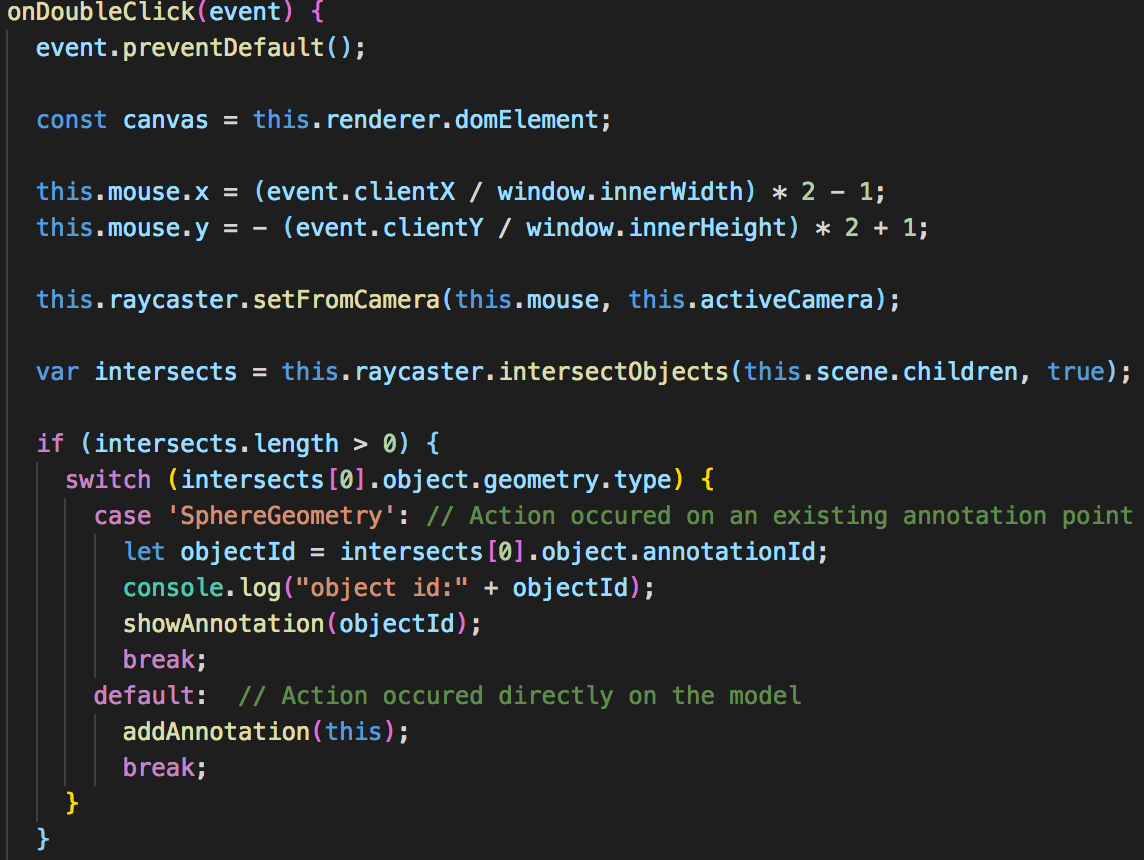
\includegraphics[width=0.8\linewidth]{Figures/mip-viewer-raycasting-code.png}
    \caption{Extrait de code illustrant les opérations effectuées pour \textit{mapper} les coordonnées 2D de l'endroit cliqué, aux coordonnées 3D correspondantes dans la scène.}
    \label{fig:mip-viewer-raycasting-code}
\end{figure}

\section{Stockage}

Il faut distinguer deux catégories d'éléments à stocker : les modèles 3D, et les annotations.
En effet, les annotations ne sont pas ajoutées directement à un modèle; les données de ce dernier ne sont jamais modifiées. Cela permet de conserver une séparation entre les deux, évite les risques de corruption des données du modèle, etc.

\subsection{Stockage des modèles 3D}

Une première possibilité d'implémentation consiste en un simple stockage des documents 3D dans le système de fichiers de la machine hébergeant la plateforme (le serveur, par exemple). Cela a notamment l'avantage d'être relativement aisé à mettre en place, car ne dépendant pas d'outils tiers complexes, et de faciliter l'importation et l'exportation des fichiers de modèle -- ceux-ci restant dans leur forme d'origine.
Dans le cadre d'un prototype

Une autre solution serait d'utiliser une base de données compatible, voire un \textit{SIG}. 
Un \textit{SIG} est un système d'information destiné à gérer des données spatiales ou géographiques. Il est difficile d'en donner une définition exacte, car les domaines concernés sont très vastes.

De manière générale, un \textit{SIG} sert à recueillir, stocker, analyser, éditer, partager et afficher lesdites données. Des outils sont mis à disposition des utilisateurs afin d'effectuer les tâches correspondantes, telles des requêtes sur les données.

\subsection{Stockage des annotations}
Les annotations pourraient être stockées, ou du moins leur propriétés, dans un fichier texte amélioré, par exemple au format \textit{JSON}.

Le contenu textuel des annotations pourrait être intégré directement dans ce document. Pour le reste, il s'agirait de références vers les emplacements des contenus avancés (images, vidéos,...). Ces médias pourraient être stockés sur le serveur, à l'instar des modèles 3D.

A noter qu'un format plus spécifique existe, mais ne semble pas encore très répandu.
\textit{GeoJSON} est un format ouvert,  basé sur JSON et défini dans une \textit{RFC}\cite{geojson-rfc}, développé pour représenter des caractéristiques géographiques. 
Celles-ci incluent les points, les lignes et les polygones ainsi que des sous-ensembles de ces types. À ces éléments, on peut ajouter des attributs.

Enfin, une autre méthode consisterait à employer un système de base de données, par exemple basé document comme \textit{MongoDB}, pour stocker les différents médias associés à une annotation, ainsi que le fichier décrivant cette dernière et contenant les références.

\section{Hébergement et déploiement}

Bien souvent, la mise en place de l'infrastructure destinée à héberger une application est fastidieuse.

Lors de la phase de développement, un déploiement local peut suffire. Évidemment, quand il s'agit de passer en production, il est nécessaire d'avoir un environnement robuste, et en l'occurence accessible depuis le web.

Les services de l'urbanisme ont généralement déjà une installation en place, pour leur \textit{SIG} par exemple. Il pourrait alors être intéressant de voir dans quelle mesure ce projet pourrait s'intégrer à un système existant plus large.

Si l'on souhaite éviter d'avoir à installer et gérer soi-même la plateforme d'hébergement, il existe heureusement d'autres solutions, notamment grâce au \textit{cloud}.

\subsection{Déploiement en continu avec Heroku}

\textit{Heroku} est une plateforme \textit{cloud} en tant que service (\textit{\textbf{P}latform \textbf{a}s \textbf{a} \textbf{S}ervice}, \textit{PaaS}) qui offre l'infrastructure nécessaire au déploiement d'applications web. Ainsi, l'équipe de développement peut se concentrer sur le logiciel lui-même sans avoir à gérer la mise en place de serveurs, leur configuration etc.

Parmi les fonctionnalités proposées :
\begin{itemize}
    \item Possibilité de mettre à jour l'application automatiquement au moindre changement dans un \textit{repository} distant, par exemple si le projet est hébergé sur \textit{GitHub},
    \item Scalabilité des processus : en cas de montée en charge (augmentation du nombre de connexions, de traitements à effectuer...), le service offre la possibilité d'allouer des ressources supplémentaires
    \item Isolation : chaque processus est isolé des autres; ainsi si l'un pose problème, le reste du produit n'est pas impacté.
    \item Des logs complets et clairs pour dépanner efficacement son application,
    \item Une documentation vaste, de nombreuses ressources pour démarrer rapidement
\end{itemize}


\textit{Heroku} n'est évidemment pas la seule enterprise à proposer ce genre de services. Ses concurrents comptent principalement \textit{Amazon Web Services (AWS)}, \textit{Windows Azure} ou encore \textit{Google App Engine}.

\textit{Heroku} se démarque quelque peu de la concurrence grâce à la relative rapidité à laquelle on peut mettre en place une première application.

Dans le cadre de la réalisation du prototype de démonstration du présent projet, l'idée était de mettre celui-ci à disposition du public en employant ce service. Malheureusement tout ne s'est pas déroulé comme prévu.

\subsubsection{Problèmes rencontrés}

\textit{Heroku} considère que l'application à déployer se situe à la racine du répertoire du projet. Or, dans le cas présent, celle-ci se trouve dans un sous-dossier, comme décrit dans l'annexe \ref{AppendixA}.

Une solution est d'employer le module \texttt{subtree} de git, qui permet de créer une sous-arborescence au sein d'un même projet. Celle-ci pourra alors être lié à une branche distincte, dont elle sera la racine. En d'autres termes, cela permet de créer une branche qui représente l'intérieur d'un répertoire.

La commande :
\begin{minted}{bash}
    git subtree push --prefix mip-viewer origin heroku
\end{minted}

crée une sous-arborescence à partir du répertoire \texttt{mip-viewer}, rattachée à la branche \texttt{heroku}.

Cependant, même après cela, d'autres soucis ont fait leur apparition. 
Tout d'abord, \textit{Heroku} étant un environnement de production (et non pas développement), des erreurs apparaissaient à l'exécution, car certaines dépendances du projet n'étaient référencées. En consultant le fichier \texttt{package.json}, celles-ci apparaissent effectivement que sous \texttt{devDependencies}. Une technique simple pour y remédier consiste à copier les entrées correspondantes sous la section \texttt{dependencies}.

Après toutes ces péripéties, \textit{Heroku} a pu générer une première \textit{build}  de l'application. Hélas, son fonctionnement reste imparfait. Il n'a alors pas été donné suite, afin de se concentrer sur d'autres parties du projet.